\providecommand{\setflag}{\newif \ifwhole \wholefalse}
\setflag
\ifwhole\else

% Typography and geometry ----------------------------------------------------
\documentclass[letterpaper]{scrbook}
\usepackage[inner=3cm,top=2.5cm,outer=3.5cm]{geometry}

\renewcommand\familydefault{bch}
\usepackage[utf8]{inputenc}
\usepackage{microtype}
\usepackage[small]{caption}
\usepackage[small]{titlesec}
\raggedbottom

% Graphics -------------------------------------------------------------------
\usepackage[pdftex]{graphicx}
\graphicspath{{_include/}}
\DeclareGraphicsExtensions{.png,.pdf}

% Code formatting ------------------------------------------------------------
\usepackage{fancyvrb}
\usepackage{courier}
\usepackage{listings}
\usepackage{color}
\usepackage{alltt}


\definecolor{comment}{rgb}{0.60, 0.60, 0.53}
\definecolor{background}{rgb}{0.97, 0.97, 1.00}
\definecolor{string}{rgb}{0.863, 0.066, 0.266}
\definecolor{number}{rgb}{0.0, 0.6, 0.6}
\definecolor{variable}{rgb}{0.00, 0.52, 0.70}
\lstset{
  basicstyle=\ttfamily,
  keywordstyle=\bfseries, 
  identifierstyle=,  
  commentstyle=\color{comment} \emph,
  stringstyle=\color{string},
  showstringspaces=false,
  columns = fullflexible,
  backgroundcolor=\color{background},
  mathescape = true,
  escapeinside=&&,
  fancyvrb
}
\newcommand{\code}[1]{\lstinline!#1!}
\newcommand{\f}[1]{\lstinline!#1()!}



% Links ----------------------------------------------------------------------

\usepackage{hyperref}
\definecolor{slateblue}{rgb}{0.07,0.07,0.488}
\hypersetup{colorlinks=true,linkcolor=slateblue,anchorcolor=slateblue,citecolor=slateblue,filecolor=slateblue,urlcolor=slateblue,bookmarksnumbered=true,pdfview=FitB}
\usepackage{url}

% Tables ---------------------------------------------------------------------
\usepackage{longtable}
\usepackage{booktabs}

% Miscellaneous --------------------------------------------------------------
\usepackage{pdfsync}
\usepackage{appendix}

\usepackage[round,sort&compress,sectionbib]{natbib}
\bibliographystyle{plainnat}


\title{ggplot2}
\author{Hadley Wickham}

\begin{document}
\fi

\chapter{Scales, axes and legends}
\label{cha:scales}

% SET_DEFAULTS
%   GG-WIDTH: 4  GG-HEIGHT: 4
%   TEX-WIDTH: 0.33\linewidth COL: 3 
%   INLINE: FALSE
%   CACHE: TRUE
% 

% END

\section{Introduction}

Scales control the mapping from data to aesthetics. They take your data and turn it into something that you can perceive visually: e.g., size, colour, position or shape. Scales also provide the tools you use to read the plot: the axes and legends (collectively known as guides). Formally, each scale is a function from a region in data space (the domain of the scale) to a region in aesthetic space (the range of the range). The domain of each scale corresponds to the range of the variable supplied to the scale, and can be continuous or discrete, ordered or unordered. The range consists of the concrete aesthetics that you can perceive and that R can understand: position, colour, shape, size and line type. If you blinked when you read that scales map data both to position and colour, you are not alone. The notion that the same kind of object is used to map data to positions and symbols strikes some people as unintuitive. However, you will see the logic and power of this notion as you read further in the chapter.

The process of scaling takes place in three steps, transformation, training and mapping, and is described in Section~\ref{sec:how-scales-work}. Without a scale, there is no way to go from the data to aesthetics, so a scale is required for every aesthetic used on the plot. It would be tedious to manually add a scale every time you used a new aesthetic, so whenever a scale is needed \ggplot will add a default. You can generate many plots without knowing how scales work, but understanding scales and learning how to manipulate them will give you much more control. Default scales and how to override them are described in Section~\ref{sec:scale-usage}. 

Scales can be roughly divided into four categories: position scales, colour scales, the manual discrete scale and the identity scale. The common options and most important uses are described in Section~\ref{sec:scale-details}. The section focusses on giving you a high-level overview of the options available, rather than expanding on every detail in depth.  Details about individual parameters are included in the online documentation.

The other important role of each scale is to produce a {\bf guide} that allows the viewer to perform the inverse mapping, from aesthetic space to data space, and read values off the plot. For position aesthetics, the axes are the guides; for all other aesthetics, legends do the job. Unlike other plotting systems, you have little direct control over the axis or legend: there is no \f{gglegend} or \f{ggaxis} to call to modify legends or axes.  Instead, all aspects of the guides are controlled by parameters of the scale. Axes and legends are discussed in Section~\ref{sec:guides}.

% Add example showing an axis and legend(s?) for the same variable mapped to different aesthetics

Section~\ref{sec:scale-resources} concludes the chapter with pointers to other academic work that discusses some of the things you need to keep in mind when assigning variables to aesthetics.

\section{How scales work}
\label{sec:how-scales-work}

To describe how scales work, we will first describe the domain (the data space) and the range (the aesthetic space), and then outline the process by which one is mapped to the other.

Since an input variable is either discrete or continuous, the domain is either a set of values (stored as a factor, character vector or logical vector) \indexf{Discrete variables} or an interval on the real line (stored as a numeric vector of length 2). For example, in the mammals sleep dataset (\code{msleep}), the domain of the discrete variable \var{vore} is \{carni, herbi, omni\}, and the domain of the continuous variable \var{bodywt} is $[0.005, 6654]$.  We often think of these as data ranges, but here we are focussing on their nature as input to the scale, i.e., as a domain of a function. \index{Data!msleep@\texttt{msleep}}

The range can also be discrete or continuous. For discrete scales, it is a vector of aesthetic values corresponding to the input values. For continuous scales, it is a 1d path through some more complicated space. For example, a colour gradient interpolates linearly from one colour to another. The range is either specified by the user when the scale is created, or by the scale itself.

The process of mapping the domain to the range includes the following stages:

\begin{itemize}

  \item {\bf transformation}: (for continuous domain only). It is often useful to display a transformation of the data, such as a logarithm or square root. Transformations are described in more depth in Section~\ref{sub:scale-position}. \index{Scales!transformation}

  After any transformations have been applied, the statistical summaries for each layer are computed based on the transformed data. This ensures that a plot of $\log(x)$ vs. $\log(y)$ on linear scales looks the same as $x$ vs. $y$ on log scales.

  \item {\bf training}:  During this key stage, the domain of the scale is learned.  Sometimes learning the domain of a scale is extremely straightforward: In a plot with only one layer, representing only raw data, it consists of determining the minimum and maximum values of a continuous variable (after transformation), or listing the unique levels of a categorical variable.  However, often the domain must reflect multiple layers across multiple datasets in multiple panels.  For example, imagine a scale that will be used to create an axis; the minimum and maximum values of the raw data in the first layer and the statistical summary in the second layer are likely to be different, but they must all eventually be drawn on the same plot. \index{Scales!training}

  The domain can also be specified directly, overriding the training process, by manually setting the domain of the scale with the {\tt limits} argument, as described in Section~\ref{sec:scale-usage}.  Any values outside of the domain of the scale will be mapped to \code{NA}.

  \item {\bf mapping:}  We now know the domain and we already knew the range before we started this process, so the last thing to do is to apply the scaling function that maps data values to aesthetic values.  \index{Scales!mapping}

\end{itemize}

We have left a few stages out of this description of the process for simplicity.  For example, we haven't discussed the role faceting plays in training, and we have also ignored position adjustments.  Nevertheless this description is accurate, and you should come back to it if you are confused about what scales are doing in your plot.

\section{Usage}
\label{sec:scale-usage}

Every aesthetic has a default scale that is added to the plot whenever you use that aesthetic. These are listed in Table~\ref{tbl:default-scales}. The scale depends on the variable type: continuous (numeric) or discrete (factor, logical, character). If you want to change the default scales see \f{set_default_scale}, described in Section~\ref{sub:customise-scales}. 

Default scales are added when you initialise the plot and when you add new layers. This means it is possible to get a mismatch between the variable type and the scale type if you later modify the underlying data or aesthetic mappings. When this happens you need to add the correct scale yourself. The following example illustrates the problem and solution. \index{Scales!defaults}

% LISTING
% 
% plot <- qplot(cty, hwy, data = mpg)
% plot
% 
% # This doesn't work because there is a mismatch between the
% # variable type and the default scale
% plot + aes(x = drv)
% 
% # Correcting the default manually resolves the problem.
% plot + aes(x = drv) + scale_x_discrete()
\input{_include/caa8c99b4e75c33bc20e5293c357df38.tex}
% END

To add a different scale or to modify some features of the default scale, you must construct a new scale and then add it to the plot using \code{+}. \indexc{+} All scale constructors have a common naming scheme.  They start with \code{scale_}, followed by the name of the aesthetic (e.g., \code{colour_}, \code{shape_} or \code{x_}), and finally by the name of the scale (e.g., \code{gradient}, \code{hue} or \code{manual}). For example, the name of the default scale for the colour aesthetic based on discrete data is {\tt scale\_colour\_hue()}, and the name of the Brewer colour scale for fill colour is {\tt scale\_fill\_brewer()}. \index{Scales!adding}

\begin{table}
  \begin{center}
  \begin{tabular}{p{1in}p{1in}p{1in}}
    \toprule
    Aesthetic & Discrete & Continuous \\
    \midrule
    Colour and fill & brewer \newline grey \newline \textbf{hue} \newline identity \newline manual & \textbf{gradient} \newline gradient2 \newline gradientn \\[0.5em]
    Position (x, y) & \textbf{discrete} & \textbf{continuous}\newline date \\[0.5em]
    Shape & \textbf{shape} \newline identity \newline manual  \\[0.5em]
    Line type & \textbf{linetype} \newline identity \newline manual \\[0.5em]
    Size & identity \newline manual & \textbf{size} \\
    \bottomrule
  \end{tabular}
  \end{center}
  \caption{Scales, by aesthetic and variable type.  Default scales are emboldened. The default scale varies depending on whether the variable is continuous or discrete.  Shape and line type do not have a default continuous scale; size does not have a default discrete scale.}
  \label{tbl:default-scales}
\end{table}

The following code illustrates this process.  We start with a plot that uses the default colour scale, and then modify it to adjust the appearance of the legend, and then use a different colour scale.  The results are shown in Figure~\ref{fig:scale-adjust}.

% FIGLISTING
%   LABEL: scale-adjust
%   CAPTION: Adjusting the default parameters of a scale. (Top left) The 
%   plot with default scale.  (Top right) Adding the default scale by hand
%   doesn't change the appearance of the plot.  (Bottom left) Adjusting the
%   parameters of the scale to tweak the legend.  (Bottom right) Using a 
%   different colour scale: Set1 from the ColorBrewer colours.
%   GG-WIDTH: 4 TEX-WIDTH: 0.5\linewidth COL: 2
% 
% p <- qplot(sleep_total, sleep_cycle, data = msleep, colour = vore)
% p 
% # Explicitly add the default scale
% p + scale_colour_hue()
% 
% # Adjust parameters of the default, here changing the appearance 
% # of the legend
% p + scale_colour_hue("What does\nit eat?", 
%    breaks = c("herbi", "carni", "omni", NA), 
%    labels = c("plants", "meat", "both", "don't know"))
% 
% # Use a different scale
% p + scale_colour_brewer(pal = "Set1")
\input{_include/306bd23706720b1692999c1095337c2e.tex}
% END

% As well as referring to scales explicitly by name, you can also refer to the default scales by their type:  {\tt discrete} or {\tt continuous}.  For example, the default discrete colour scale (hue) can be referred to as \code{scale_colour_discrete}.  
% 
% Having to specify the type of variable (continuous or discrete) seems like extra work: why can't ggplot2 figure that out by itself?  Well, it can't because you can create the scales independently of (and before) the plot.  Allows you to create scales independently of the plot.  

\section{Scale details}
\label{sec:scale-details}

Scales can be divided roughly into four separate groups:

\begin{itemize}
  \item Position scales, used to map continuous, discrete and date-time variables onto the plotting region and to construct the corresponding axes.

  \item Colour scales, used to map continuous and discrete variables to colours.

  \item Manual scales, used to map discrete variables to your choice of symbol size, line type, shape or colour, and to create the corresponding legend.

  \item The identity scale, used to plot variable values directly to the aesthetic rather than mapping them.  For example, if the variable you want to map to symbol colour is itself a vector of colours, you want to render those values directly rather than mapping them to some other colours.

\end{itemize}

\noindent  This section describes each group in more detail.  Precise details about individual scales can be found in the documentation, within R (e.g., {\tt ?scale\_brewer}), or online at  \url{http://had.co.nz/ggplot2}.  

\subsection{Common arguments}
\label{sub:scale-arguments}

The following arguments are common to all scales.

\begin{itemize}
  \item {\tt name}:  sets the label which will appear on the axis or legend. You can supply text strings (using \verb|\n| for line breaks) or mathematical expressions (as described by \verb|?plotmath|).  Because tweaking these labels is such a common task, there are three helper functions to save you some typing: \f{xlab}, \f{ylab} and \f{labs}.  Their use is demonstrated in the code below and results are shown in Figure~\ref{fig:legend-names}. \index{Axis!labels} \index{Legend!title} \index{Scales!names}

  % FIGLISTING
  %  LABEL: legend-names 
  %  CAPTION: A demonstration of the different forms legend title can take.
  %  TEX-WIDTH: 0.33\linewidth
  %  COL: 3
  % 
  % p <- qplot(cty, hwy, data = mpg, colour = displ)
  % p
  % p + scale_x_continuous("City mpg")
  % p + xlab("City mpg")
  % p + ylab("Highway mpg")
  % p + labs(x = "City mpg", y = "Highway", colour = "Displacement")
  % p + xlab(expression(frac(miles, gallon)))
  \input{_include/a69d51d7a4dcdc9b5f817da3a989a1d1.tex}  
  % END

  \item {\tt limits}: fixes the domain of the scale.   Continuous scales take a numeric vector of length two; discrete scales take a character vector. If limits are set, no training of the data will be performed.  See Section~ \ref{sub:scale-position} for shortcuts. \index{Axis!limits} \index{Scales!limits}
  
  Limits are useful for removing data you don't want displayed in a plot (i.e., setting limits that are smaller than the full range of data), and for ensuring that limits are consistent across multiple plots intended to be compared (i.e., setting limits that are larger or smaller than some of the default ranges).  
  
  Any value not in the domain of the scale is discarded: for an observation to be included in the plot, each aesthetic must be in the domain of each scale.  This discarding occurs before statistics are calculated. 
  
  \item {\tt breaks} and {\tt labels}: {\tt breaks} controls which values appear on the axis or legend, i.e., what values tick marks should appear on an axis or how a continuous scale is segmented in a legend. {\tt labels} specifies the labels that should appear at the breakpoints. If {\tt labels} is set, you must also specify {\tt breaks}, so that the two can be matched up correctly. \index{Axis!breaks} \index{Axis!labels} \index{Legend!keys}

  To distinguish breaks from limits, remember that breaks affect what appears on the axes and legends, while limits affect what appears on the plot.  See Figure~\ref{fig:breaks_vs_limits} for an illustration.  The first column uses the default settings for both breaks and limits, which are {\tt limits = c(4, 8)} and {\tt breaks = 4:8}.  In the middle column, the breaks have been reset: the plotted region is the same, but the tick positions and labels have shifted.  In the right column, it is the limits which have been redefined, so much of the data now falls outside the plotting region. 
  
  % FIGLISTING
  %   LABEL: breaks_vs_limits
  %   COL: 3 TEX-WIDTH: 0.33\linewidth
  %   CAPTION: The difference between breaks and limits.  (Left) 
  %   default plot with {\tt limits = c(4, 8), breaks = 4:8}, (middle)  
  %   {\tt breaks = c(5.5,6.5)} and (right) {\tt limits = c(5.5,6.5)}.
  %   The effect on the x axis (top) and colour legend (bottom)
  % 
  % p <- qplot(cyl, wt, data = mtcars)
  % p
  % p + scale_x_continuous(breaks = c(5.5, 6.5))
  % p + scale_x_continuous(limits = c(5.5, 6.5))
  % p <- qplot(wt, cyl, data = mtcars, colour = cyl)
  % p
  % p + scale_colour_gradient(breaks = c(5.5, 6.5))
  % p + scale_colour_gradient(limits = c(5.5, 6.5))
  \input{_include/9e99b27b669b2329b2e3df4d0902237d.tex}  
  % END

  \item {\bf formatter}: if no labels are specified the formatter will be called on each break to produce the label.  Useful formatters for continuous scales are \code{comma}, \code{percent}, \code{dollar} and \code{scientific}, and for discrete scales is \code{abbreviate}. \index{Axis!formatting}
\end{itemize}

\subsection{Position scales}
\label{sub:scale-position}

Every plot must have two position scales, one for the horizontal position (the x scale) and one for the vertical position (the y scale). \ggplot comes with continuous, discrete (for factor, character and logical vectors) and date scales. Each of these transform the data in a slightly different way, and generate a slightly different type of axis. The following sections describe each type in more detail. \index{Scales!position} \index{Positioning!scales}

A common task for all position axes is changing the axis limits.  Because this is such a common task, \ggplot provides a couple of helper functions to save you some typing: \f{xlim} and \f{ylim}.  These functions inspect their input and then create the appropriate scale, as follows: \index{Axis!limits} \index{Scales!limits} \indexf{xlim}  \indexf{ylim} \index{Limits|see{Axis, limits}}

\begin{itemize}
  \item \code{xlim(10, 20)}: a continuous scale from 10 to 20
  \item \code{ylim(20, 10)}: a reversed continuous scale from 20 to 10
  \item \code{xlim("a", "b", "c")}: a discrete scale
  \item \code{xlim(as.Date(c("2008-05-01", "2008-08-01")))}: a date scale from May 1 to August 1 2008.
\end{itemize}

These limits do not work in the same way as \code{xlim} and \code{ylim} in base or lattice graphics.  In \ggplot, to be consistent with the other scales, any data outside the limits is not plotted and not included in the statistical transformation.  This means that setting the limits is not the same as visually zooming in to a region of the plot.  To do that, you need to use the \code{xlim} and \code{ylim} arguments to \f{coord_cartesian}, described in Section~\ref{sub:cartesian}.  This performs purely visual zooming and does not affect the underlying data. \index{Zooming}

 % Position scales also have the {\bf expand} argument, which controls the amount of extra space added to axis limits.  This is a numeric vector of length two: the first number is a multiplicative amount and the second is an additive constant.  The default for continuous scales is {\tt c(0.05, 0)} (i.e.,\ add 5\% extra space on each end); for discrete scales it is {\tt c(0, 0.75)}).  Set to {\tt c(0, 0)} to eliminate extra space.

By default, the limits of position scales extend a little past the range of the data. This ensures that the data does not overlap the axes. You can control the amount of expansion with the \code{expand} argument. This parameter should be a numeric vector of length two. The first element gives the multiplicative expansion, and the second the additive expansion.  If you don't want any extra space, use \code{expand = c(0, 0)}. \index{Axis!expansion}

\subsubsection{Continuous}
\label{sub:scale-continuous}

The most common continuous position scales are {\tt scale\_x\_continuous} and {\tt scale\_y\_continuous}, which map data to the x and y axis. \index{Scales!position!continuous} The most interesting variations are produced using transformations.  Every continuous scale takes a {\tt trans} argument, allowing the specification of a variety of transformations, both linear and non-linear.  The transformation is carried out by a ``transformer,'' which describes the transformation, its inverse, and how to draw the labels. Table~\ref{tbl:common-trans} lists some of the more common transformers. \index{Transformation!scales} \indexf{scale_x_continuous} \indexf{scale_y_continuous} \index{Scales!continuous}

\begin{table}
  \centering
  \begin{tabular}{lll}
    \toprule
    Name & Function $f(x)$ & Inverse $f^{-1}(y)$ \\
    \midrule
    asn       & $\tanh^{-1}(x)$ & $\tanh(y)$ \\
    exp       & $e ^ x$         & $\log(y)$  \\
    identity  & $x$             & $y$        \\
    log       & $\log(x)$       & $e ^ y$    \\
    log10     & $\log_{10}(x)$  & $10 ^ y$   \\
    log2      & $\log_2(x)$     & $2 ^ y$    \\
    logit     & $\log(\frac{x}{1 - x})$ & $\frac{1}{1 + e(y)} $ \\
    pow10     & $10^x$          & $\log_{10}(y) $ \\
    probit    & $\Phi(x)$       & $\Phi^{-1}(y)$ \\
    recip     & $x^{-1}$        & $y^{-1}$ \\
    reverse   & $-x$            & $-y$     \\
    sqrt      & $x^{1/2}$       & $y ^ 2$  \\
    % power     & $\frac{x^p - 1}{p * sgn(values - 1)}$ & $|values| * p + 1 $ 
    \bottomrule
  \end{tabular}
  \caption{List of built-in transformers.}
  \label{tbl:common-trans}
\end{table}

Transformations are most often used to modify position scales, so there are shortcuts for x, y and z scales: \f{scale_x_log10} is equivalent to \verb|scale_x_continuous(trans = "log10")|.  The \code{trans} argument works for any continuous scale, including the colour gradients described below, but the shortcuts only exist for position scales. \index{Log transform} \indexf{scale_x_log10} \indexf{scale_y_log10}

Of course, you can also perform the transformation yourself. For example, instead of using \f{scale_x_log}, you could plot {\tt log10(x)}. That produces an identical result inside the plotting region, but the the axis and tick labels won't be the same. If you use a transformed scale, the axes will be labelled in the original data space. In both cases, the transformation occurs before the statistical summary. Figure~\ref{fig:trans} illustrates this difference with the following code. \index{Transformation!data}

% FIGLISTING
%   FILETYPE: PNG
%   LABEL: trans
%   CAPTION: A scatterplot of diamond price vs.\ carat illustrating the
%   difference between log transforming the scale (left) and log transforming
%   the data (right).  The plots are identical, but the axis labels are
%   different.
% 
% qplot(log10(carat), log10(price), data = diamonds)
% qplot(carat, price, data = diamonds) + 
%   scale_x_log10() + scale_y_log10()
\input{_include/1c8f49e21277d92dabd9fffe944f3b89.tex}
% END

Transformers are also used in \f{coord_trans}, where the transformation occurs after the statistic has been calculated, and affects the shape of the graphical object drawn on the plot. \f{coord_trans} is described in more detail in Section\ref{sub:cartesian}.

\subsubsection{Date and time}
\label{sub:scale-date}

Dates and times are basically continuous values, but with special ways of labelling the axes. Currently, only dates of class \code{date} and times of class \code{POSIXct} are supported. If your dates are in a different format you will need to convert them with \f{as.Date} or \f{as.POSIXct}.  \index{Date} \index{Time} \index{Scales!date-time} \indexf{scale_x_datetime}

There are three arguments that control the appearance and location of the ticks for date axes: \code{major}, \code{minor} and \code{format}. Generally, the scale does a pretty good job of choosing the defaults, but if you need to tweak them the details are as follows:

\begin{itemize}
  \item The \code{major} and \code{minor} arguments specify the position of major and minor breaks in terms of date units, years, months, weeks, days, hours, minutes and seconds, and can be combined with a multiplier.  For example, \code{major = "2 weeks"} will place a major tick mark every two weeks.  If not specified, the date scale has some reasonable default for choosing them automatically.
  
  \item The \code{format} argument specifies how the tick labels should be formatted. Table~\ref{tbl:dates} lists the special characters used to display components of a date.  For example, if you wanted to display dates of the form 14/10/1979, you would use the string \verb|"%d/%m/%y"|. \index{Time series!date formatting}
\end{itemize}

\begin{table}
  \begin{center}
  \begin{tabular}{ll}
    \toprule
    Code & Meaning \\
    \midrule
    \verb|%S| & second (00-59)\\
    \verb|%M| & minute (00-59)\\
    \verb|%l| & hour, in 12-hour clock (1-12)\\
    \verb|%I| & hour, in 12-hour clock (01-12)\\
    \verb|%H| & hour, in 24-hour clock (00-23)\\
    \verb|%a| & day of the week, abbreviated (Mon-Sun)\\
    \verb|%A| & day of the week, full (Monday-Sunday)\\
    \verb|%e| & day of the month (1-31)\\
    \verb|%d| & day of the month (01-31)\\
    \verb|%m| & month, numeric (01-12)\\
    \verb|%b| & month, abbreviated (Jan-Dec)\\
    \verb|%B| & month, full (January-December)\\
    \verb|%y| & year, without century (00-99)\\
    \verb|%Y| & year, with century (0000-9999)\\
    \bottomrule
    
  \end{tabular}
  \end{center}
  \caption{Common data formatting codes, adapted from the documentation of \code{strptime}.  Listed from shortest to longest duration.}
  \label{tbl:dates}
\end{table}

The code below generates the plots in Figure~\ref{fig:date-scale}, illustrating some of these parameters.

% FIGLISTING
%   LABEL: date-scale
%   CAPTION: A time series of personal savings rate.  (Left) The default
%   appearance, (middle) breaks every 10 years, and (right) scale restricted
%   to 2004, with YMD date format.  Measurements are recorded at the end of 
%   each month.
% 
% plot <- qplot(date, psavert, data = economics, geom = "line") + 
%   ylab("Personal savings rate") +
%   geom_hline(xintercept = 0, colour = "grey50")
% plot
% plot + scale_x_date(major = "10 years")
% plot + scale_x_date(
%   limits = as.Date(c("2004-01-01", "2005-01-01")),
%   format = "%Y-%m-%d"
% )
\input{_include/12a8f20c035e934db2b075e96cd02418.tex}
% END

\subsubsection{Discrete}
\label{sub:scale-discrete}

Discrete position scales map the unique values of their input to integers.  The order of the result can be controlled by the \code{breaks} argument, and levels can be dropped with the \code{limits} argument (or by using \f{xlim} or \f{ylim}).  Because it is often useful to place labels and other annotations on intermediate positions on the plot, discrete position scales also accept continuous values.  If you have not adjusted the breaks or limits, the numerical position of a factor level can be calculated with \f{as.numeric}: the values are placed on integers starting at 1. \index{Scales!position!discrete} \indexf{scale_x_discrete} \indexf{scale_y_discrete} \index{Scales!discrete}

% TODO: think of a better example to put here
%% FIGLISTING
%% 
%% japanese <- subset(mpg, manufacturer %in% 
%%   c("toyota", "honda", "nissan", "subaru", "hyundai"))
%% qplot(hwy, manufacturer, data = japanese) + 
%%   geom_text(aes(y = as.numeric(factor(manufacturer)) - 0.1, label = model), 
%%    size = 2, angle = -45, hjust = 0, stat = "unique")
%% 

\subsection{Colour}
\label{sub:scale-colour}

After position, probably the most commonly used aesthetic is colour. There are quite a few different ways of mapping values to colours: three different gradient based methods for continuous values, and two methods for mapping discrete values. But before we look at the details of the different methods, it's useful to learn a little bit of colour theory. Colour theory is complex because the underlying biology of the eye and brain is complex, and this introduction will only touch on some of the more important issues. An excellent more detailed exposition is available online at \url{http://tinyurl.com/clrdtls}. \index{Colour} \index{Scales!colour}

At the physical level, colour is produced by a mixture of wavelengths of lights. To know a colour completely we need to know the complete mixture of wavelengths, but fortunately for us the human eye only has three different colour receptors, and so we can summarise any colour with just three numbers. You may be familiar with the rgb encoding of colour space, which defines a colour by the intensities of red, green and blue light needed to produce it. One problem with this space is that it is not perceptually uniform: the two colours that are one unit apart may look similar or very different depending on where in the colour space they. This makes it difficult to create a mapping from a continuous variable to a set of colours.  There have been many attempts to come up with colours spaces that are more perceptually uniform.  We'll use a modern attempt called the hcl colour space, which has three components of {\bf h}ue, {\bf c}hroma and {\bf l}uminance: \index{Colour!spaces}

\begin{itemize}
  \item Hue is a number between 0 and 360 (an angle) which gives the ``colour'' of the colour: like blue, red, orange, etc.
  \item Luminance is the lightness of the colour.  A luminance of 0 produces black, and a luminance of 1 produces white.
  \item Chroma is the purity of a colour.  A chroma of 0 is grey, and the maximum value of chroma varies with luminance.
\end{itemize} 

The combination of these three components does not produce a simple geometric shape.  Figure~\ref{fig:hcl} attempts to show the 3d shape of the space.  Each slice is a constant luminance (brightness) with hue mapped to angle and chroma to radius.  You can see the centre of each slice is grey and the colours get more intense as they get closer to the edge.

\begin{figure}[htbp]
  \centering
    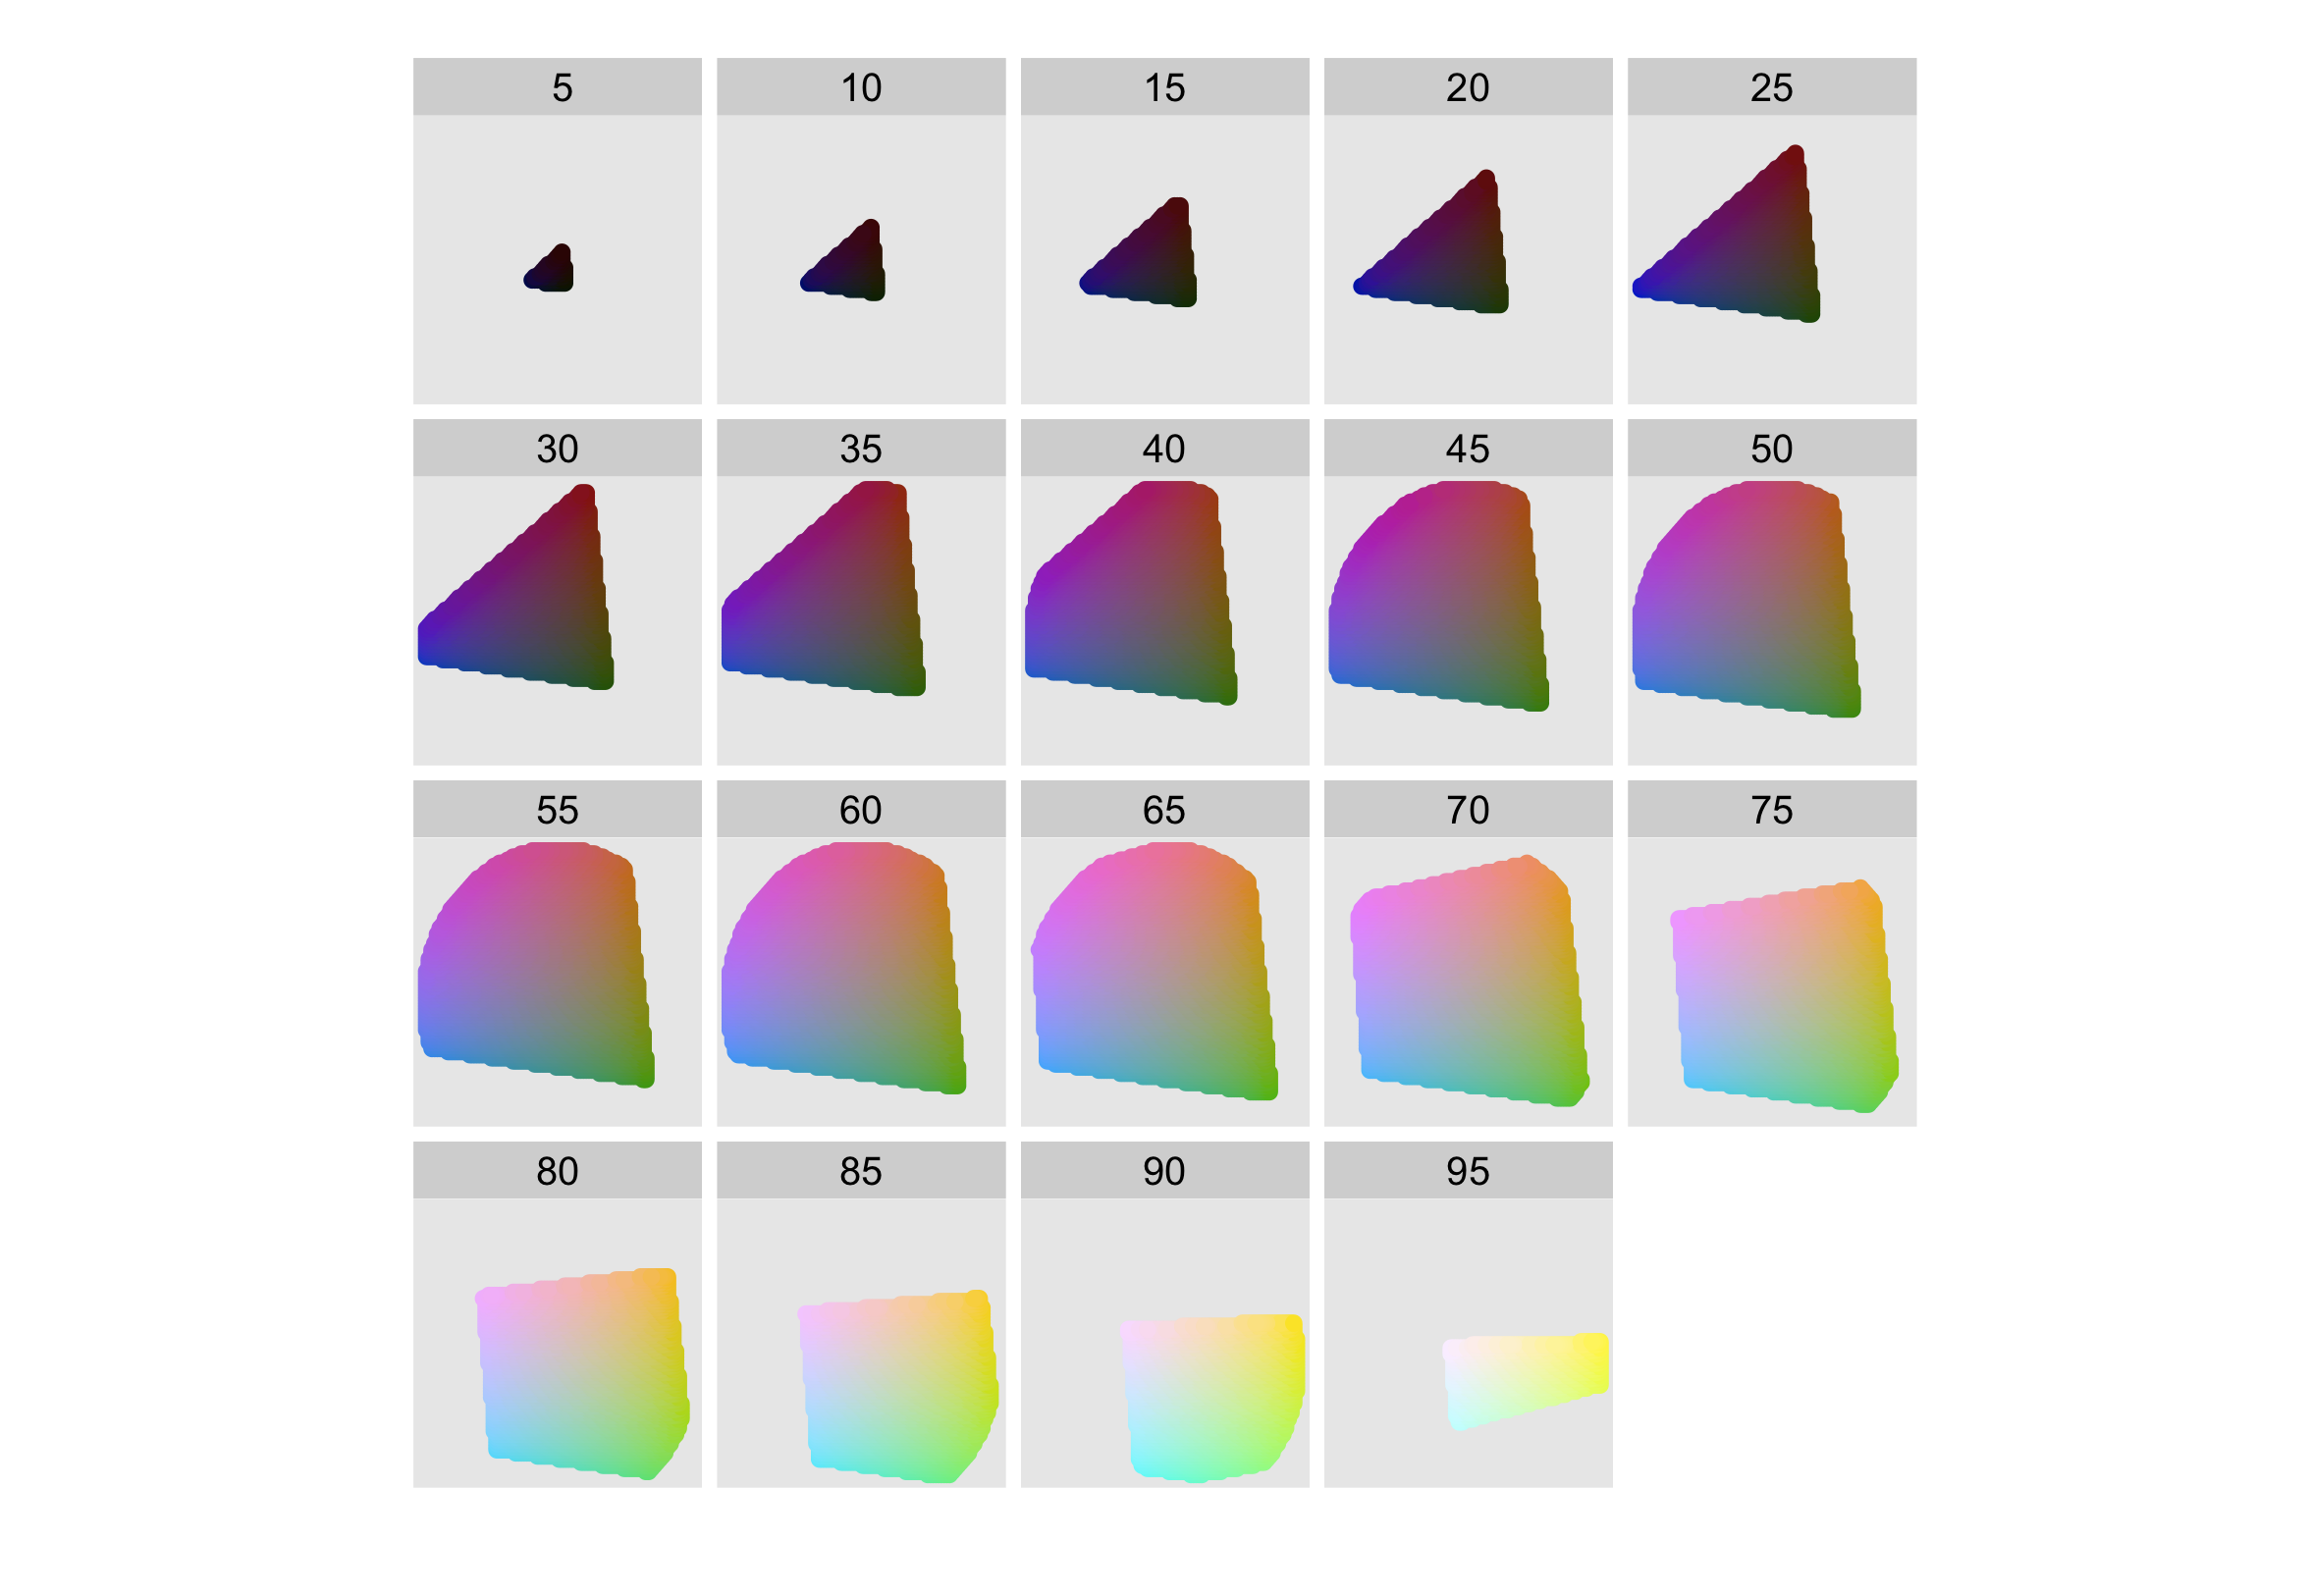
\includegraphics[width=\linewidth]{hcl-space}
  \caption{The shape of the hcl colour space.  Hue is mapped to angle, chroma to radius and each slice shows a different luminance.  The hcl space is a pretty odd shape, but you can see that colours near the centre of each slice are grey, and as you move towards the edges they become more intense.  Slices for luminance 0 and 100 are omitted because they would, respectively, be a single black point and a single white point.}
  \label{fig:hcl}
\end{figure}

An additional complication is that many people ($\sim$10\% of men) do not possess the normal complement of colour receptors and so can distinguish fewer colours than usual. \index{Colour!blindness} In brief, it's best to avoid red-green contrasts, and to check your plots with systems that simulate colour blindness. Visicheck is one online solution. Another alternative is the dichromat package \citep{dichromat} which provides tools for simulating colour blindness, and a set of colour schemes known to work well for colour-blind people. You can also help people with colour blindness in the same way that you can help people with black-and-white printers: by providing redundant mappings to other aesthetics like size, line type or shape.

All of the scales discussed in the following sections work with border (\code{colour}) and fill (\code{fill}) colour aesthetics.

% \url{http://cran.r-project.org/web/packages/dichromat}
% http://casoilresource.lawr.ucdavis.edu/drupal/node/201
% http://colororacle.cartography.ch/

\subsubsection{Continuous}
\label{ssub:colour-continuous}

There are three types of continuous colour gradients, based on the number of colours in the gradient: \index{Colour!gradients} \index{Scales!colour!gradient}

\begin{itemize}
  \item \f{scale_colour_gradient} and \f{scale_fill_gradient}: a two-colour gradient, low-high.  Arguments \code{low} and \code{high} control the colours at either end of the gradient. \indexf{scale_colour_gradient} \indexf{scale_fill_gradient}

  \item \f{scale_colour_gradient2} and \f{scale_fill_gradient2}: a three-colour gradient, low-med-high.  As well as \code{low} and \code{high} colours, these scales also have a \code{mid} colour for the colour of the midpoint.  The midpoint defaults to 0, but can be set to any value with the \code{midpoint} argument.  This is particularly useful for creating diverging colour schemes.\indexf{scale_colour_gradient2} \indexf{scale_fill_gradient2}

  \item \f{scale_colour_gradientn} and \f{scale_fill_gradientn}: a custom n-colour gradient.  This scale requires a vector of colours in the \code{colours} argument.  Without further arguments these colours will be evenly spaced along the range of the data.  If you want the values to be unequally spaced, use the \code{values} argument, which should be between 0 and 1 if \code{rescale} is true (the default), or within the range of the data is \code{rescale} is false. 
\end{itemize}

Colour gradients are often used to show the height of a 2d surface.  In the following example we'll use the surface of a 2d density estimate of the \code{faithful} dataset \citep{azzalini:1990}, which records the waiting time between eruptions and during each eruption for the Old Faithful geyser in Yellowstone Park. Figure~\ref{fig:gradient} shows three gradients applied to this data, created with the following code.  Note the use of limits: this parameter is common to all scales.

% FIGLISTING
%   LABEL: gradient
%   FILETYPE: png
%   CAPTION: Density of eruptions with three colour schemes.  (Left) Default
%   gradient colour scheme, (middle) customised gradient from white to black
%   and (right) 3 point gradient with midpoint set to the mean density.
% 
% f2d <- with(faithful, MASS::kde2d(eruptions, waiting, 
%   h = c(1, 10), n = 50))
% df <- with(f2d, cbind(expand.grid(x, y), as.vector(z)))
% names(df) <- c("eruptions", "waiting", "density")
% erupt <- ggplot(df, aes(waiting, eruptions, fill = density)) +
%   geom_tile() +
%   scale_x_continuous(expand = c(0, 0)) + 
%   scale_y_continuous(expand = c(0, 0))
% erupt + scale_fill_gradient(limits = c(0, 0.04))
% erupt + scale_fill_gradient(limits = c(0, 0.04), 
%   low = "white", high = "black") 
% erupt + scale_fill_gradient2(limits = c(-0.04, 0.04), 
%   midpoint = mean(df$density)) 
\input{_include/0e6317869cd0afa4cbed69fa22f7b69f.tex}
% END

% http://www.vendian.org/mncharity/dir3/blackbody/

To create your own custom gradient, use \f{scale_colour_gradientn}. This is useful if you have colours that are meaningful for your data (e.g., black body colours or standard terrain colours), or you'd like to use a palette produced by another package. The following code and Figure~\ref{fig:vcd} shows palettes generated from routines in the \code{vcd} package. \citet{zeileis:2008} describes the philosophy behind these palettes and provides a good introduction to some of the complexities of creating good colour scales. \index{Colour!palettes} \indexf{scale_colour_gradientn} \indexf{scale_fill_gradientn}

% FIGLISTING 
%   LABEL: vcd
%   FILETYPE: png
%   CAPTION: Gradient colour scales using perceptually well-formed palettes
%   produced by the \code{vcd} package.  From left to right: sequential,
%   diverging and heat hcl palettes.  Each scale is produced with 
%   \code{scale_fill_gradientn} with \code{colours} set to 
%   \code{rainbow_hcl(7)}, \code{diverge_hcl(7)} and \code{heat_hcl(7)}.
% 
% library(vcd)
% fill_gradn <- function(pal) {
%   scale_fill_gradientn(colours = pal(7), limits = c(0, 0.04))
% }
% erupt + fill_gradn(rainbow_hcl)
% erupt + fill_gradn(diverge_hcl)
% erupt + fill_gradn(heat_hcl)
\input{_include/293f949c45aaa2c891a98b6679677bfc.tex}
% END

\subsubsection{Discrete}
\label{ssub:colour-discrete}

There are two colour scales for discrete data, one which chooses colours in an automated way, and another which makes it easy to select from hand-picked sets.

The default colour scheme, \f{scale_colour_hue}, picks evenly spaced hues around the hcl colour wheel.  This works well for up to about eight colours, but after that it becomes hard to tell the different colours apart.  Another disadvantage of the default colour scheme is that because the colours all have the same luminance and chroma, when you print them in black and white, they all appear as an identical shade of grey. \index{Colour!discrete scale} \indexf{scale_colour_hue}

An alternative to this algorithmic scheme is to use the ColorBrewer colours, \url{http://colorbrewer.org}. These colours have been hand picked to work well in a wide variety of situations, although the focus is on maps and so the colours tend to work better when displayed in large areas. For categorical data, the palettes most of interest are ``Set1'' and ``Dark2'' for points and ``Set2'', ``Pastel1'', ``Pastel2'' and ``Accent'' for areas. Use {\tt RColorBrewer::display.brewer.all} to list all palettes. Figure~\ref{fig:brewer-pal} shows three of these palettes applied to points and bars, created with the following code.  \index{Colour!Brewer} \indexf{scale_colour_brewer}

% FIGLISTING
%   LABEL: brewer-pal
%   CAPTION: Three ColorBrewer palettes, Set1 (left), Set2 (middle) and
%   Pastel1 (right), applied to points (top) and bars (bottom).
%   Bright colours work well for points, but are overwhelming on bars.  
%   Subtle colours work well for bars, but are hard to see on points.
% 
% point <- qplot(brainwt, bodywt, data = msleep, log = "xy", 
%   colour = vore)
% area <- qplot(log10(brainwt), data = msleep, fill = vore, 
%   binwidth = 1)
% 
% point + scale_colour_brewer(pal = "Set1")
% point + scale_colour_brewer(pal = "Set2")
% point + scale_colour_brewer(pal = "Pastel1")
% area + scale_fill_brewer(pal = "Set1")
% area + scale_fill_brewer(pal = "Set2")
% area + scale_fill_brewer(pal = "Pastel1")
\input{_include/56ba05c208ebb130274c1f478741911f.tex}
% END

If you have your own discrete colour scale, you can use \f{scale_colour_manual}, as described below.

\subsection{The manual discrete scale}
\label{sub:scale-manual}

The discrete scales, \f{scale_linetype}, \f{scale_shape} and {\tt scale\-\_size\-\_discrete} basically have no options (although for the shape scale you can choose whether points should be filled or solid). These scales are just a list of valid values that are mapped to each factor level in turn. \index{Shape!scale} \index{Line type!scale} \index{Size!scale}

If you want to customise these scales, you need to create your own new scale with the manual scale: \f{scale_shape_manual}, \f{scale_linetype_manual}, \f{scale_colour_manual}, etc. The manual scale has one important argument, \verb|values|, where you specify the values that the scale should produce. If this vector is named, it will match the values of the output to the values of the input, otherwise it will match in order of the levels of the discrete variable. You will need some knowledge of the valid aesthetic values, which are described in Appendix \ref{cha:specifications}.  The following code demonstrates the use of \f{scale_manual}, with results shown in Figure~\ref{fig:scale-manual} \indexf{scale_shape_manual} \indexf{scale_colour_manual} \indexf{scale_linetype_manual}

% FIGLISTING
%   LABEL: scale-manual
%   CAPTION: Scale manual used to create custom colour (left and middle) and
%   shape (right) scales.
% 
% plot <- qplot(brainwt, bodywt, data = msleep, log = "xy")
% plot + aes(colour = vore) + 
%   scale_colour_manual(value = c("red", "orange", "yellow", 
%     "green", "blue"))
% colours <- c(carni = "red", "NA" = "orange", insecti = "yellow", 
%   herbi = "green", omni = "blue")
% plot + aes(colour = vore) + scale_colour_manual(value = colours)
% plot + aes(shape = vore) + 
%   scale_shape_manual(value = c(1, 2, 6, 0, 23))
\input{_include/2ab94c5487d14c916981c8e9a4c04cd2.tex}
% END

The following example shows a creative use \f{scale_colour_manual}, when you want to display multiple variables on the same plot, and show a useful legend. In most other plotting systems, you'd just colour the lines as below, and then add a legend that describes which colour corresponds to which variable.  That doesn't work in \ggplot because it's the scales that are responsible for drawing legends, and the scale doesn't know how the lines should be labelled.

% INTERWEAVE  
%   TEX-WIDTH: 0.75\linewidth
%   GG-WIDTH: 7
% 
% huron <- data.frame(year = 1875:1972, level = LakeHuron)
% ggplot(huron, aes(year)) +
%   geom_line(aes(y = level - 5), colour = "blue") + 
%   geom_line(aes(y = level + 5), colour = "red")
\input{_include/318ee0bc7edd7dd94d740bfda0698346.tex}
% END

What you need to do is tell the colour scale about the two different lines by creating a mapping from the data to the colour aesthetic. There's no variable present in the data, so you'll have to create one:

% INTERWEAVE  
%   TEX-WIDTH: 0.75\linewidth
%   GG-WIDTH: 7
% 
% ggplot(huron, aes(year)) +
%   geom_line(aes(y = level - 5, colour = "below")) + 
%   geom_line(aes(y = level + 5, colour = "above"))
\input{_include/a64c85497d4a7e9764be503a76f6bddc.tex}
% END

This gets us basically what we want, but the legend isn't labelled correctly, and has the wrong colours.  That can be fixed with \code{scale_colour_manual}:

% INTERWEAVE  
%   TEX-WIDTH: 0.75\linewidth
%   GG-WIDTH: 7
% 
% ggplot(huron, aes(year)) +
%   geom_line(aes(y = level - 5, colour = "below")) + 
%   geom_line(aes(y = level + 5, colour = "above")) + 
%   scale_colour_manual("Direction", 
%     c("below" = "blue", "above" = "red"))
\input{_include/ef0c01da1949157aac507d489fcba43d.tex}
% END

See Section~\ref{sub:time-series} for an alternative approach to the problem.

\subsection{The identity scale}
\label{sub:scale-identity}

The identity scale is used when your data is already in a form that the plotting functions in R understand, i.e., when the data and aesthetic spaces are the same.  This means there is no way to derive a meaningful legend from the data alone, and by default a legend is not drawn.  If you want one, you can still use the \code{breaks} and \code{labels} arguments to set it up yourself. \index{Scales!identity} \indexf{scale_identity}

Figure~\ref{fig:scale-identity} shows one sort of data where \code{scale_identity} is useful.  Here the data themselves are colours, and there's no way we could make a meaningful legend.  The identity scale can also be useful in the case where you have manually scaled the data to aesthetic values.  In that situation, you will have to figure out what breaks and labels make sense for your data.

% FIGURE
%   LABEL: scale-identity
%   COL: 1 TEX-WIDTH: 0.5\linewidth
%   CAPTION: A plot of R colours in Luv space.  A legend is unnecessary,
%   because the colour of the points represents itself: the data and aesthetic
%   spaces are the same.
% 
% x <- colors()
% luv <- as.data.frame(convertColor(t(col2rgb(x)), "sRGB", "Luv"))
% qplot(u, v, data=luv, colour = x, size = I(3)) + scale_colour_identity() +
%    coord_equal()
\input{_include/71867429de64edd13098035ba1402e4f.tex}
% END

\section{Legends and axes}
\label{sec:guides}

Collectively, axes and legends are called {\bf guides}, and they are the inverse of the scale: they allow you to read observations from the plot and map them back to their original values.  Figure~\ref{fig:labelled-guides} labels the guides and their components.  There are natural equivalents between the legend and the axis: the legend title and axis label are equivalent and determined by the scale name; the legend keys and tick labels are both determined by the scale breaks. \index{Guides}

\begin{figure}[htbp]
  \centering
  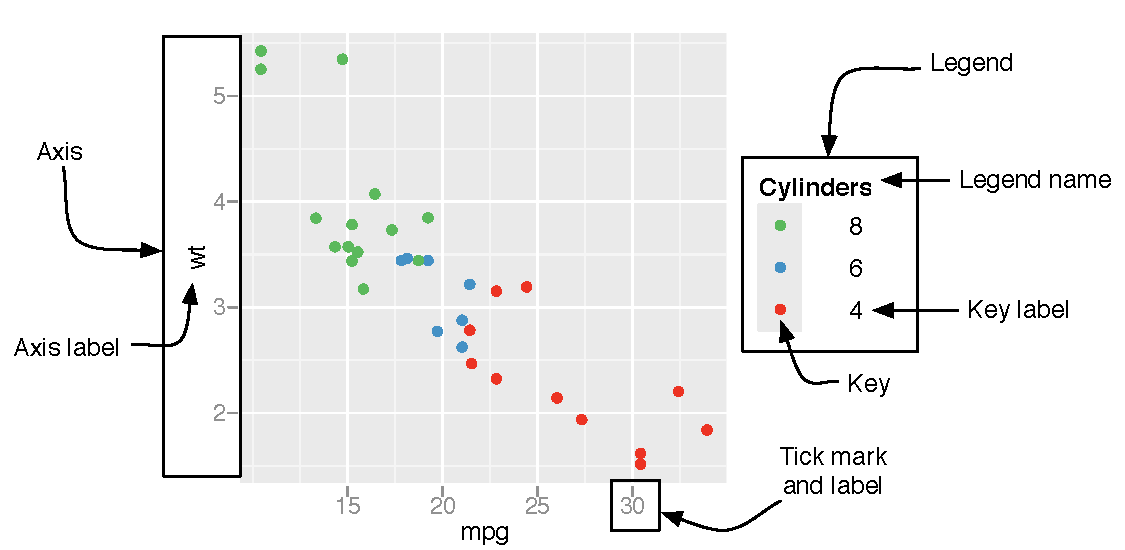
\includegraphics[width=\linewidth]{scale-guides}
  
  \caption{The components of the axes and legend.}
  \label{fig:labelled-guides}
\end{figure}

In \ggplot, legends and axes are produced automatically based on the scales and geoms that you used in the plot. This is different than how legends work in most other plotting systems, where you are responsible for adding them.  In \ggplot, there is little you can do to directly control the legend.  \index{Legend} This seems like a big restriction at first, but as you get more comfortable with this approach, you will discover that it saves you a lot of time, and there is little you cannot do with it.

To draw the legend, the plot must collect information about how each aesthetic is used: for what data and what geoms. The scale breaks are used to determine the values of the legend keys and a list of the geoms that use the aesthetic  is used to determine how to draw the keys. For example, if you use the point geom, then you will get points in the legend; if you use the lines geom, you will get lines. If both point and line geoms are used, then both points and lines will be drawn in the legend.  This is illustrated in Figure~\ref{fig:legend-geom}.

% FIGURE
%   TEX-WIDTH: 1in  GG-WIDTH: 1.5 GG-HEIGHT: 2
%   LABEL: legend-geom
%   CAPTION: Legends produced by geom: point, line, point and line, and bar.
% 
% p <- ggplot(diamonds[1:100, ], aes(price, carat, colour = cut)) +  
%   opts(keep = "legend_box")
% p + geom_point()
% p + geom_line()
% p + geom_point() + geom_line()
% p + geom_bar(binwidth = 100) + aes(fill = cut, y = ..count..)
\input{_include/5f16085df8873e2ae61180105aee019a.tex}
% END

\ggplot tries to use the smallest possible number of legends that accurately conveys the aesthetics used in the plot.  It does this by combining legends if a variable is used with more than one aesthetic.  Figure~\ref{fig:legend-merge} shows an example of this for the points geom: if both colour and shape are mapped to the same variable, then only a single legend is necessary.  In order for legends to be merged, they must have the same name (the same legend title).  For this reason, if you change the name of one of the merged legends, you'll need to change it for all of them.

% FIGURE
%   TEX-WIDTH: 1in  GG-WIDTH: 1.5 GG-HEIGHT: 2
%   LABEL: legend-merge
%   CAPTION: Colour legend, shape legend, colour + shape legend. 
% 
% p <- ggplot(diamonds[1:100, ], aes(price, carat)) +  
%   geom_point() + 
%   opts(keep = "legend_box")
% p + aes(colour = cut)
% p + aes(shape = cut)
% p + aes(shape = cut, colour = cut)
\input{_include/f78cfefa65a2144fb366808f7fd48ec1.tex}
% END

The contents of the legend and axes are controlled by the scale, and the details of the rendering are controlled by the theming system. The following list includes the most commonly tweaked settings.

\begin{itemize}
  \item The scale {\tt name} controls the axis label and the legend title.  This can be a string, or a mathematical expression, as described in \code{?plotmath}.
  
  \item The {\tt breaks} and {\tt labels} arguments to the scale function, introduced earlier in this chapter, are particularly important because they control what tick marks appear on the axis and what keys appear on the legend.  If the breaks chosen by default are not appropriate (or you want to use more informative labels), setting these arguments will adjust the appearance of the legend keys and axis ticks.  \index{Legend!keys}
  
  \item The theme settings {\tt axis.*} and {\tt legend.*} control the visual appearance of axes and legends.  To learn how to manipulate these settings, see Section~\ref{sec:themes}.

  \item The internal grid lines are controlled by the breaks and minor breaks arguments.  By default minor grid lines are spaced evenly in the original data space: this gives the common behaviour of log-log plots where major grid lines are multiplicative and minor grid lines are additive.  You can override the minor grid lines with the {\tt minor\_breaks} argument.  Grid line appearance is controlled by the \code{panel.grid.major} and \code{panel.grid.minor} theme settings. \index{Grid}

  \item The position and justification of legends are controlled by the theme setting {\tt legend.position}, and the value can be right, left, top, bottom, none (no legend), or a numeric position.  The numeric position gives (in values between 0 and 1) the position of the corner given by {\tt legend.justification}, a numeric vector of length two.  Top right = \code{c(1, 1)}, bottom left = \code{c(0, 0)}. \index{Legend!position}
  
\end{itemize}

\section{More resources}
\label{sec:scale-resources}

As you experiment with different aesthetic choices and new scales, it's important to keep in mind how the plot will be perceived.   Some particularly good references to consult are:

\begin{itemize}
  \item \citet{cleveland:1993,cleveland:1987,cleveland:1994} for research on how plots are perceived and the best ways to encode data.
  \item \citet{tufte:2006,tufte:1990,tufte:1997,tufte:2001} for how to make beautiful, data-rich, graphics.
  \item \citet{brewer:1994,brewer:1994a} for how to choose colours that work well in a wide variety of situations, particularly for area plots.
  \item \citet{carr:1999,carr:1994,carr:2002} for the use of colour in general.
\end{itemize}

\ifwhole
\else
  \nobibliography{/Users/hadley/documents/phd/references}
  \end{document}
\fi
